\documentclass[main]{subfiles}
\begin{document}

\section*{Lecture 8 // Sept 17 // Singularities in $\mc{M}$ \& Holonomy}
\addcontentsline{toc}{section}{Lecture 8 -- Singularities in M and Holonomy}

\textbf{Last Time:} Let $(M^4,g)$ be positive definite and simply connected. Fix a $k=1$ $\SU(2)$ bundle $E$ over $M$. Consider $\mc{M}=\mc{A}/\mc{G}$ the SDYM moduli space. We know the following qualitative features of $\mc{M}$:
\begin{enumerate}
\item Away from a finite number of singular points, $\mc{M}$ is a smooth $5$-dimensional oriented manifold.
\item The number of these points $=$ the number of splittings of $E$.
\item Each point has a neighborhood homeomorphic to the cone on $\CP^2$; diffeomorphic away from the point.
\item $\mc{M}$ is not compact, but it admits a compactification $\overline{\mc{M}}$ such that $\partial\overline{\mc{M}}\cong M$.
\end{enumerate}

\begin{center}
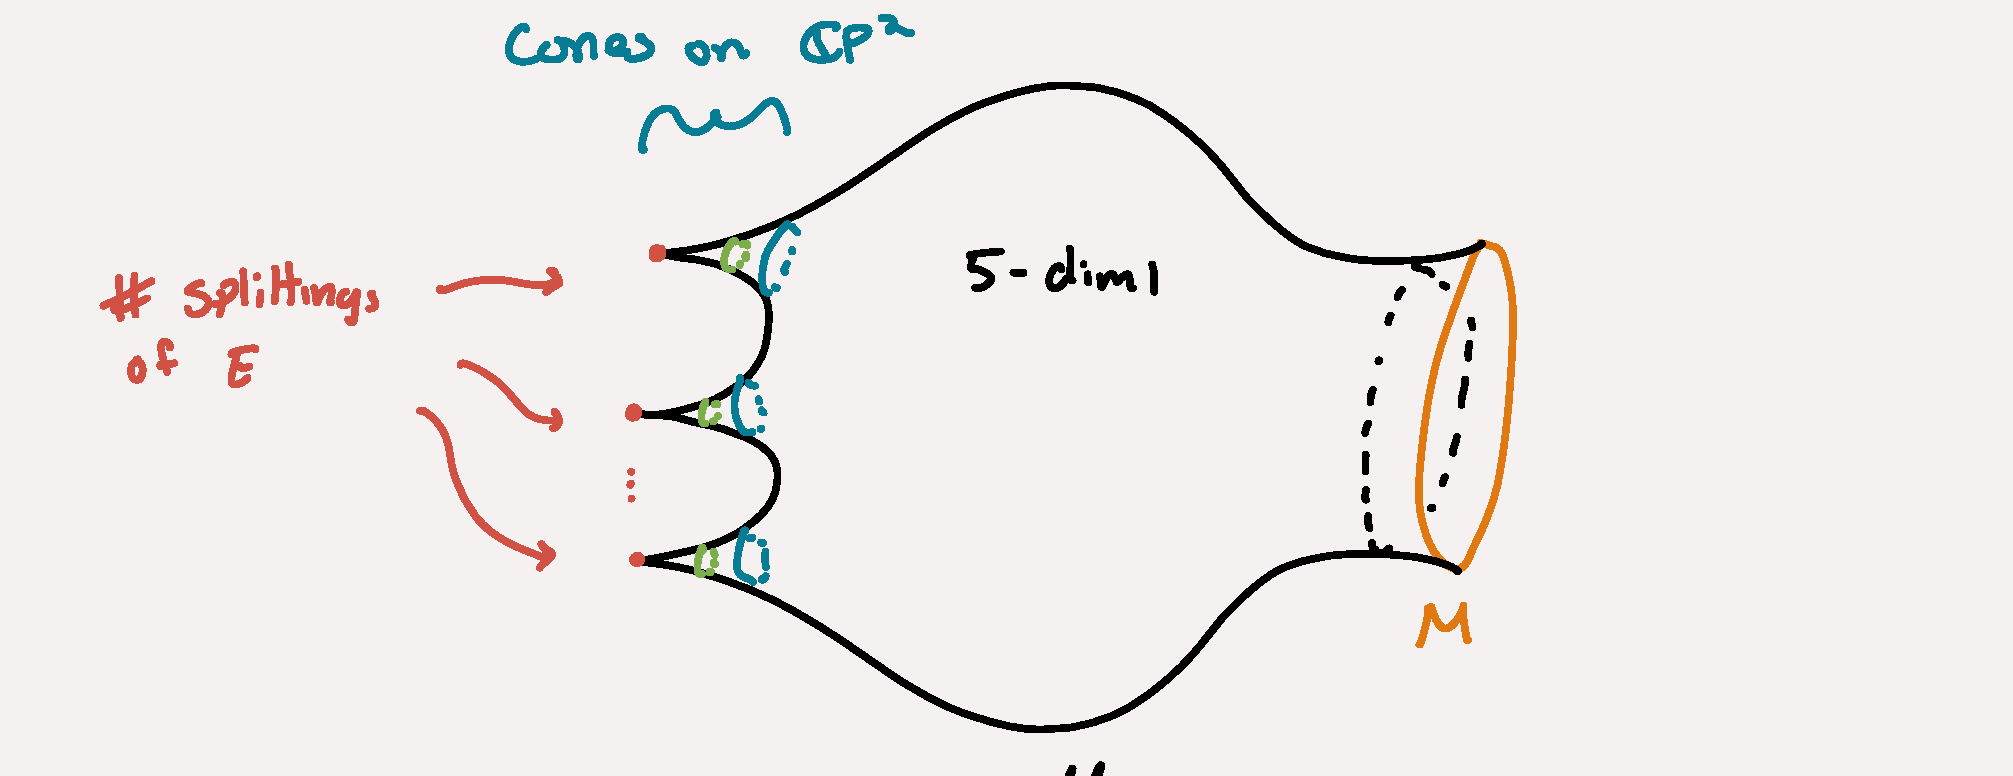
\includegraphics[width=0.9\linewidth]{figures/fig_lec8_mbar.png}
\end{center}

After some linear algebra, these properties prove Donaldson's theorem: since $\sigma$ is a bordism invariant,
\[
\underbrace{\operatorname{rk} Q_M}_{\text{since definite}} = \sigma(M) = \#\text{ splittings of } E = \frac{1}{2}\#\{x\in H_2 \text{ with } x^2=1\}.
\]

Today, we'll unpack these points: why is $\mc{M}$ singular, and why do neighborhoods look like the cone on $\CP^2$?

\subsection*{Singularities in $\mc{M}$}

Recall that $\mc{M} = \{\text{SDYM conn.}\}/\mc{G}$. $\{\text{SDYM conn.}\}\subseteq \mc{A}$, which is a smooth manifold, on which $\mc{G}$ acts. However, $\mc{G}$ may have stabilizer subgroups. Thus the singularities arise from the failure of $\mc{G}$ to act freely on $\mc{A}$.

\begin{remark}
Establishing $\{\text{SDYM conn.}\}$ is a smooth manifold is fairly standard: it is the zero locus of a map from an $\infty$-dimensional manifold to somewhere else; verify that $0$ is a regular value, apply Sard-Smale.
\end{remark}

\begin{definition}
For $\nabla\in\mc{A}$, $\Stab(\nabla) = \{g\in\mc{G} \mid g^\ast(\nabla)=\nabla\}$,
\[
A\longrightarrow g^{-1}Ag + g^{-1}dg.
\]
\end{definition}

What can $\Stab(\nabla)$ be? First note that for every $\nabla$, $\pm\mathrm{Id}\in\Stab(\nabla)$. Since $\pm\mathrm{Id}$ is sent to itself under conjugation, $\pm\mathrm{Id}$ is a well-defined section of $\Aut(E)$. These are not interesting gauge transformations, so it's sometimes more convenient to take $\mc{G}/\pm\mathrm{Id} \curvearrowright \mc{A}$ instead.

What else is possible? Let's examine an example. Connections with nontrivial stabilizers are related to the number of splittings. For a line bundle $L$, consider the constant gauge transformation given by multiplication by a fixed element of $S^1$, $e^{i\theta}\in S^1$. For $E = L\oplus \bar{L}$, consider now
\[
g = \begin{pmatrix} e^{i\theta} & 0 \\ 0 & e^{-i\theta}\end{pmatrix}.
\]
One can check this is a well-defined gauge transformation on $E$. If $\nabla$ is split, e.g., $A = \begin{pmatrix} ia & 0 \\ 0 & -ia\end{pmatrix}$, easy to check that $g^\ast(\nabla)=\nabla$. So if $E$ is split and $\nabla$ is a split connection, considered as a subgroup of $\SU(2)$, $\Stab(\nabla)$ is at least as big as $S^1$.

\begin{remark}
In this observation, we play fast and loose with the difference between a local definition of a gauge transformation and its definition globally. The correct statement is given in the following lemma, and the tension between global \& local will be resolved as we introduce the tools to prove it.
\end{remark}

\begin{lemma}
For an $\SU(2)$ bundle with $k\neq 0$, a connection has stabilizer bigger than $\pm\mathrm{Id}$ iff it is split, and $\Stab(\nabla)\cong S^1$.
\end{lemma}

The proof isn't hard, but requires more technical language. But this lemma gives why the singularities of $\mc{M}$ are what they are. We showed previously that each splitting of $E$ supports a unique (up to $\mc{G}$) split SDYM connection. Each singular point is the unique SDYM connection for a splitting. Thus the number of singular points is the number of splittings. This gives (2).

We now ask why local neighborhoods are cones on $\CP^2$. Near a singular point, $\mc{G}/\pm I$ acts freely. The approximate idea is that we first quotient by $\pm I$ to get a $6$-dimensional manifold with a $S^1/\pm I$ action which acts freely except at one point. The local model for this is $S^1\curvearrowright \mathbb{R}^6\cong \mathbb{C}^3$ via usual $S^1$ complex multiplication. $\mathbb{C}^3/S^1 \cong$ cone on $\CP^2$ with one singular point, since on each $S^5$ slice, we have $S^5/S^1 \cong \CP^2$ (via definition $\CP^n := S^{2n+1}/S^1$).

\begin{center}
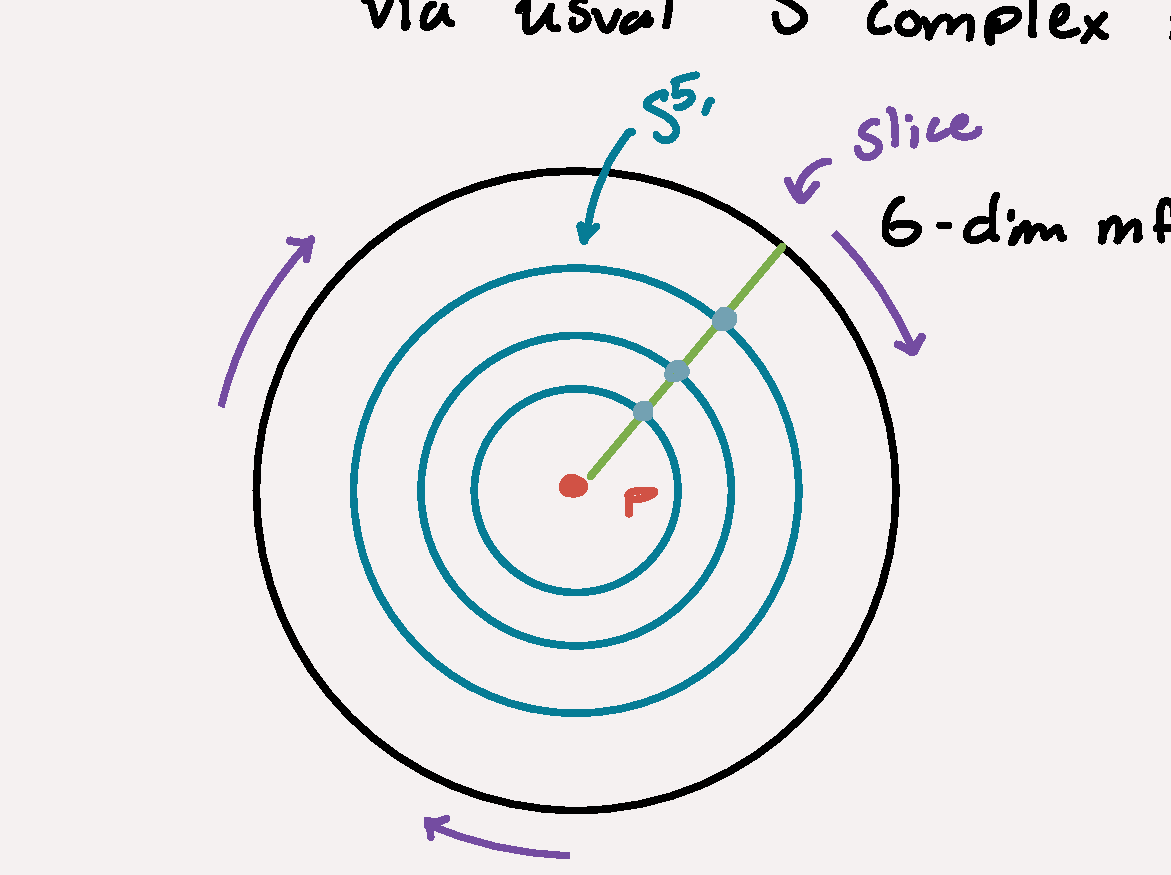
\includegraphics[width=0.5\linewidth]{figures/fig_lec8_cone_spheres.png}
\end{center}

\begin{note}
The $\pm I \subset \mc{G}$ and $S^1$ actions are more entertwined in $\mc{G}$ than this; we can't actually quotient by gauge in this ``partial'' way. But it gives an approximate idea.
\end{note}

\begin{question}
Why is $\mc{M}$ $5$-dimensional?
\end{question}
This is where we use that $k=1$. The dimension is from the Atiyah-Singer index formula applied to a Fredholm operator whose zero locus are the SDYM connections. When $k>1$, we get more generally that the singular neighborhood is $\cong$ cone on $\CP^n$.

We now must introduce more differential geometry.

\subsection*{Interlude: Parallel Transport}

Let $E$ be a vector bundle over $M$.

\begin{definition}
Let $\nabla$ be a connection on $E$, $\gamma : [0,1]\to M$ a path. A section $s$ defined along $\gamma$ is parallel transported by $\nabla$ along $\gamma$ if $\nabla_{\gamma'(t)}s = 0$ for all $t$.
\end{definition}

\begin{lemma}
Let $\gamma : [0,1]\to M$ be a path from $p$ to $q$. If we fix any $v\in E_p$, then there exists a unique section $s$ defined along $\gamma$ such that $s$ extends $v$ and $s$ is parallel transported by $\nabla$ along $\gamma$.
\end{lemma}

\begin{proof}[Proof idea]
Using the existence of solutions to ODEs, we can construct $s$ and show that $(d+A)s=0$. \qedhere
\end{proof}

To better see the point of parallel transport, we can observe the effect of parallel transport on a frame of $E_p$, i.e., a basis for $E_p$, and parallel transport that basis along $\gamma$. Parallel transport preserves orthonormality, so this gives you a particular trivialization of $E$ along $\gamma$ for which the basis elements are covariantly constant: $A$ vanishes in the path direction $\gamma'$. In essence, the covariant derivative specifies a ``preferred frame'' along each path, which we can find by choosing a frame at one end and parallel transporting it along the path.

\begin{center}
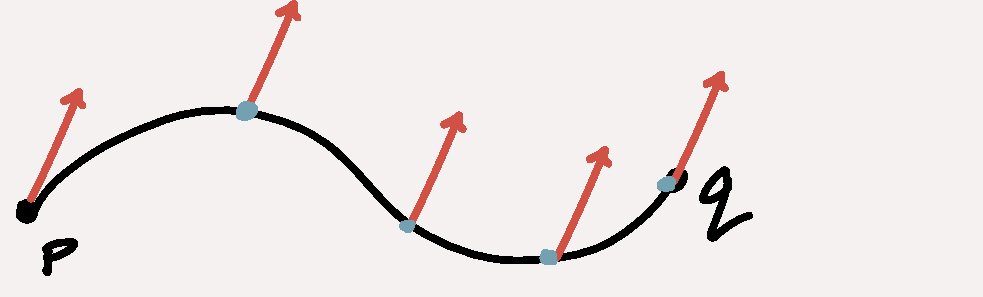
\includegraphics[width=0.6\linewidth]{figures/fig_lec8_parallel_path.png}
\end{center}

What else can parallel transport do? For each path $\gamma$ from $p$ to $q$, we can build a linear map from $E_p$ to $E_q$ which sends $v\in E_p$ to the endpoint of the parallel transport of $v$ along $\gamma$. Call this map $\hol_{p,q}(\gamma) : E_p\to E_q$. Since $\hol_{p,q}(\gamma)\circ\hol_{q,p}(\bar\gamma) = \mathrm{id}$, this map is an isomorphism.

Now, take $q=p$, so $\gamma$ is a based loop in $M$. Then $\hol_p = \hol_{p,p}$ gives a map $E_p\to E_p$, so defines an element $\hol_p(\gamma)\in \GL(E_p)$.

\begin{definition}
Holonomy is a map $\hol_p : \{\text{loops based at } p\} \to \GL(E_p)$.
\end{definition}

\textbf{Properties of Holonomy:}
\begin{enumerate}
\item If $E$ is a $G$-bundle and $\nabla$ is a $G$ connection, then $\hol_p(\gamma)$ is $G\subseteq \GL(E_p)$ valued.
\item If $F_\nabla = 0$, the holonomy only depends on the based smooth homotopy class of $\gamma$. I.e., $\hol_p$ descends to a map
\[
\hol_p : \pi_1(M) \to \GL(E_p) \quad (\text{or } G \text{ for } G).
\]
For $G = \SU(2)$, $\hol_p : \pi_1(M) \to \SU(2)$ is a $\SU(2)$ representation of $\pi_1(M)$.
\item If $g$ is a gauge transformation,
\[
\hol_{p,q}^{g^\ast(\nabla)}(\gamma) = g_q^{-1}\circ \hol_{p,q}^\nabla(\gamma)\circ g_p.
\]
\end{enumerate}

To illustrate holonomy, consider a trivial line bundle $L = M\times\mathbb{C}$ over $M$ and a $U(1)$ connection on $L$ given by $\nabla = d+ia$, $a\in \Omega^1(M;\mathbb{R})$. Thus a section here is just a $\mathbb{C}$-valued function. For a path $\gamma$, what does it mean for $\nabla_{\gamma'(t)}s=0$? Given a based loop $\gamma$ and a section defined along $\gamma$, what does it mean for $s$ to be parallel transported along $\gamma$? Since we're working in a line bundle, a section is just a $\mathbb{C}$-valued function, and for $\nabla_{\gamma'(t)}s=0$, the covariant derivative of this function must vanish along $\gamma$. Explicitly, we get
\[
\nabla_{\gamma'(t)}s = 0, \qquad (ds)(\gamma'(t)) + ia(\gamma'(t))s = 0, \qquad \frac{d}{dt}(s\circ\gamma) + ia(\gamma'(t))(s\circ\gamma(t)) = 0.
\]

But this is just a differential equation, which we can solve as usual:
\[
\frac{d}{dt}(s\circ\gamma) = -ia(\gamma'(t))(s\circ\gamma(t)) \ \Rightarrow\ (s\circ\gamma) = \left(e^{-i\int_0^t a(\gamma'(h))\,dh}\right)s(\gamma(0)).
\]
If we conflate $s$ and $s\circ\gamma$, we get that $\hol_{p,q} = e^{-i\int_\gamma a}\in S^1$.

Intuitively, we're supposed to think that solving $(d+A)s=0$ gives $s(t) = e^{-\int A}s(0)$, so if $A$ is Lie algebra valued, $-\int A$ is Lie algebra valued, so $e^{-\int A}$ is Lie group valued. In reality, this is false -- there's an issue with commutativity when $G\neq U(1)$.

However we see directly here that $\hol(\gamma)$ need not be the identity: if $\int_\gamma a\neq 2\pi n$, $e^{-i\int_\gamma a}\neq 1$.

In fact we see a nice connection with property \#3. Indeed, suppose that $\gamma$ bounds a region $R$. Then Stokes' theorem says that
\[
\int_\gamma a = \int_{\partial R} a = \int_R da,
\]
where $da$ is the curvature of $\nabla$.

\begin{center}
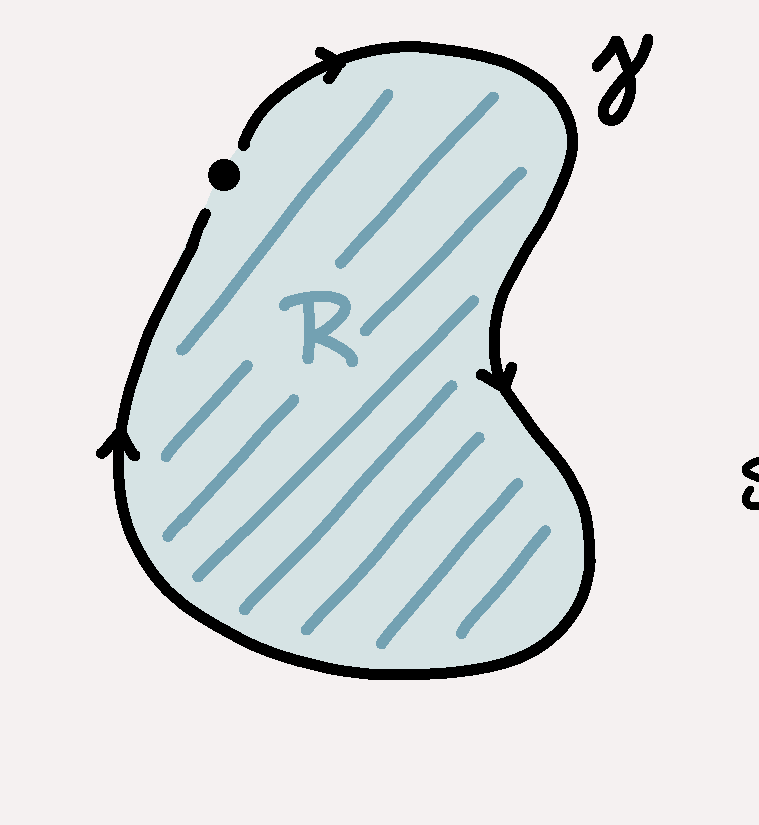
\includegraphics[width=0.4\linewidth]{figures/fig_lec8_region_loop.png}
\end{center}

So the heuristic is that holonomy picks up the curvature of a connection.

This demonstrates, in the $U(1)$ case, assertion \#3: if $\gamma$ is varied through a region where $F_\nabla=0$, then holonomy is not changed. However, note that this analysis applies to single coordinate charts; it is purely local. If the bundle is nontrivial, it is not true that $F_A=0$ implies that $\hol(\gamma)=\mathrm{id}$. Furthermore, it makes no sense to treat the differential equation like it's globally defined, since $a$ isn't. But it is true that holonomy is constant in its homotopy class.

\textbf{Next time:} We'll use parallel transport to discuss the lemma on the exact behavior of stabilizers of connections.

\end{document}
